% Created 2024-08-30 Fri 17:52
% Intended LaTeX compiler: pdflatex
\documentclass[11pt]{article}
\usepackage[utf8]{inputenc}
\usepackage[T1]{fontenc}
\usepackage{graphicx}
\usepackage{longtable}
\usepackage{wrapfig}
\usepackage{rotating}
\usepackage[normalem]{ulem}
\usepackage{amsmath}
\usepackage{amssymb}
\usepackage{capt-of}
\usepackage{hyperref}
\usepackage{minted}
\usepackage[a4paper, margin=2.5cm]{geometry}
\usepackage{minted}
\usepackage{fontspec}
\setmonofont{Iosevka}
\setminted{fontsize=\small, frame=single, breaklines=true}
\usemintedstyle{emacs}
\usepackage[backend=biber,style=apa]{biblatex}
\addbibresource{citation.bib}
\author{Baley Eccles - 652137 and Tyler Robards - 651790}
\date{\textit{{[}2024-08-26 Mon 12:08]}}
\title{ENG204 - Signals and Linear Systems – Assignment 1.2}
\hypersetup{
 pdfauthor={Baley Eccles - 652137 and Tyler Robards - 651790},
 pdftitle={ENG204 - Signals and Linear Systems – Assignment 1.2},
 pdfkeywords={},
 pdfsubject={},
 pdfcreator={Emacs 29.4 (Org mode 9.8)}, 
 pdflang={English}}
\begin{document}

\maketitle
\tableofcontents

\section{ENG204 - Signals and Linear Systems – Assignment 1.2}
\label{sec:org831f92d}
\subsection{Part a}
\label{sec:org72d9136}
Free Body Diagram
\begin{center}
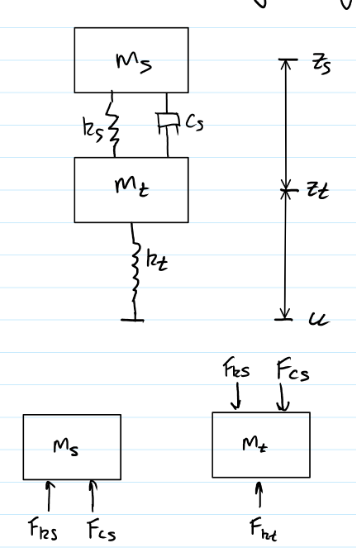
\includegraphics[width=.9\linewidth]{ENG204-FBD.png}
\end{center}
The gravational forces can be ignored because they will cause a constant downward force. Where we will only be looking at the differences in forces between the systems. In other words, the system will respond in the same way whether or not the gravitational forces are included. This is because the system that is being looked at only cares about the differences in forces, and not their total value.
\subsection{Part b}
\label{sec:orgb61511b}
\subsubsection{Differential Equation}
\label{sec:orgfba282b}
\begin{minted}[]{octave}
clc
clear
pkg load symbolic
syms mt at ms as  ...
    Fkt Fks Fcs Fks
% sum F_y = ma
eq1 = mt*at == Fkt - Fks - Fcs;
eq2 = ms*as == Fks + Fcs;


% Sub in force equations
syms kt u zt zs dzs dzt ks cs
FktEqu = kt*(u-zt);
FksEqu = ks*(zt-zs);
FcsEqu = cs*(dzt-dzs);
eq1=subs(subs(subs(eq1,Fkt,FktEqu),Fks,FksEqu),Fcs,FcsEqu);
eq2=subs(subs(subs(eq2,Fkt,FktEqu),Fks,FksEqu),Fcs,FcsEqu);
\end{minted}



Using these equations from the free body diagram:
\begin{itemize}
\item \(a_t m_t = - F_{cs} - F_{ks} + F_{kt}\)
\item \(a_s m_s = F_{cs} + F_{ks}\)
\end{itemize}
And:
\begin{itemize}
\item \(F_{kt} = k_t \left(u - z_t\right)\)
\item \(F_{ks} = k_s \left(- z_s + z_t\right)\)
\item \(F_{cs} = c_s \left(- \dot{z}_s + \dot{z}_t\right)\)
\end{itemize}
Will result in the differential equations for the system:
\begin{itemize}
\item \(a_t m_t = \dot{v_t} m_t = \ddot{z_t} m_t = -c_s \left(- \dot{z}_s + \dot{z}_t\right) - k_s \left(- z_s + z_t\right) + k_t \left(u - z_t\right)\)
\item \(a_s m_s = \dot{v_s} m_s = \ddot{z_s} m_s =  c_s \left(- \dot{z}_s + \dot{z}_t\right) + k_s \left(- z_s + z_t\right)\)
\end{itemize}
\subsubsection{Difference Equations}
\label{sec:org752e860}
Next we can create the difference equations by subsituting in the forward differences for the velocities and accelerations:
\begin{itemize}
\item \(\dot{z_s} = \frac{- z_s[n] + z_s[n+1]}{T_s}\)
\item \(\dot{z_t} = \frac{- z_t[n] + z_t[n+1]}{T_s}\)
\item \(a_s = \dot{v_s} = \frac{- v_s[n] + v_s[n+1]}{T_s}\)
\item \(a_t = \dot{v_t} = \frac{- v_t[n] + v_t[n+1]}{T_s}\)
\end{itemize}
\begin{minted}[]{octave}
% Sub in forward difference
syms zs zs1 zs2 zt zt1 zt2 Ts vs1 vt1 vs vt
% First forward difference of displacement
dzsEqu = (zs1-zs)/(Ts);
dztEqu = (zt1-zt)/(Ts);
% First forward differences of acceleration
dvsEqu = (vs1-vs)/(Ts);
dvtEqu = (vt1-vt)/(Ts);
eq1=subs(eq1,at,dvtEqu);
eq1=subs(eq1,dzs,vs);
eq1=subs(eq1,dzt,vt);
eq1=expand(simplify(eq1));
eq2=subs(eq2,as,dvsEqu);
eq2=subs(eq2,dzs,vs);
eq2=subs(eq2,dzt,vt);
eq2=expand(simplify(eq2));
\end{minted}
Which produces the two following difference equations:
\begin{itemize}
\item \(-\frac{m_t v_t[n]}{T_s} + \frac{m_t v_t[n+1]}{T_s} = c_s v_s[n] - c_s v_t[n] + k_s z_s[n] - k_s z_t[n] + k_t u[n] - k_t z_t[n]\)
\item \(-\frac{m_s v_s[n]}{T_s} + \frac{m_s v_s[n+1]}{T_s} = - c_s v_s[n] + c_s v_t[n] - k_s z_s[n] + k_s z_t[n]\)
\end{itemize}
\subsection{Part c}
\label{sec:orgd8c82cd}


We need to find the matricies of the two following equations:
\begin{itemize}
\item \(\underline{q}[n+1]=\underline{A}q[n]+\underline{b}x[n]\)
\item \(y[n]=\underline{C}q[n]+dx[n]\)
\end{itemize}
We chose the following state varibles:
\begin{itemize}
\item \(q_1[n] = z_t[n]\)
\item \(q_2[n] = v_t[n] = \dot{z_t}[n]\)
\item \(q_3[n] = z_s[n]\)
\item \(q_4[n] = v_s[n] = \dot{z_s}[n]\)
\item \(q_1[n+1] = z_t[n+1]\)
\item \(q_2[n+1] = v_t[n+1] = \dot{z_t}[n+1]\)
\item \(q_3[n+1] = z_s[n+1]\)
\item \(q_4[n+1] = v_s[n+1] = \dot{z_s}[n+1]\)
\item \(x[n] = u[n]\)
\item \(y[n] = \begin{bmatrix} z_t[n] \\ z_s[n] \end{bmatrix}\)
\end{itemize}
\subsubsection{State Equation}
\label{sec:org99c1e04}
Need to solve for the matricies in \(\underline{q}[n+1]=\underline{A}q[n]+\underline{b}x[n]\). To do this we will subsitute in the state varibles into the difference equations.
\begin{minted}[]{octave}
syms q1n q1n1 q2n q2n1 q3n q3n1 q4n q4n1

eq1 = subs(eq1,zt,q1n);
eq1 = subs(eq1,vt,q2n);
eq1 = subs(eq1,zs,q3n);
eq1 = subs(eq1,vs,q4n);
eq1 = subs(eq1,zt1,q1n1);
eq1 = subs(eq1,vt1,q2n1);
eq1 = subs(eq1,zs1,q3n1);
eq1 = subs(eq1,vs1,q4n1);

eq2 = subs(eq2,zt,q1n);
eq2 = subs(eq2,vt,q2n);
eq2 = subs(eq2,zs,q3n);
eq2 = subs(eq2,vs,q4n);
eq2 = subs(eq2,zt1,q1n1);
eq2 = subs(eq2,vt1,q2n1);
eq2 = subs(eq2,zs1,q3n1);
eq2 = subs(eq2,vs1,q4n1);

equq1n1 = q1n+Ts*q2n;
equq3n1 = q3n+Ts*q4n;

eq1 = subs(eq1, q1n1, equq1n1);
eq1 = subs(eq1, q3n1, equq3n1);
eq2 = subs(eq2, q1n1, equq1n1);
eq2 = subs(eq2, q3n1, equq3n1);

eq1 = expand(simplify(solve(eq1,q2n1)));
eq2 = expand(simplify(solve(eq2,q4n1)));
\end{minted}

Which gives us the following equations:
\begin{itemize}
\item \(q_1[n+1]=q_1[n]+T_s\cdot q_2[n]\)
\item \(q_2[n+1]=-\frac{T_s c_s q_2[n]}{m_t} + \frac{T_s c_s q_4[n]}{m_t} - \frac{T_s k_s q_1[n]}{m_t} + \frac{T_s k_s q_3[n]}{m_t} - \frac{T_s k_t q_1[n]}{m_t} + \frac{T_s k_t u[n]}{m_t} + q_2[n]\)
\item \(q_3[n+1]=q_3[n]+T_s\cdot q_4[n]\)
\item \(q_4[n+1]=\frac{T_s c_s q_2[n]}{m_s} - \frac{T_s c_s q_4[n]}{m_s} + \frac{T_s k_s q_1[n]}{m_s} - \frac{T_s k_s q_3[n]}{m_as} + q_4[n]\)
\end{itemize}
These four equations can be used to fill in the matrix \(A\) and \(B\):
\[\underline{A} = \begin{bmatrix}
1 & T_s & 0 & 0 \\
-\frac{T_s k_s }{m_t} - \frac{T_s k_t }{m_t} & 1 - \frac{T_s c_s }{m_t} & \frac{T_s k_s }{m_t} & \frac{T_s c_s }{m_t} \\
0 & 0 & 1 & T_s \\
\frac{T_s k_s }{m_s} & \frac{T_s c_s }{m_s} &  -\frac{T_s k_s }{m_s} & 1 - \frac{T_s c_s }{m_s}
\end{bmatrix}\]
\[\underline{B} = \begin{bmatrix}
0 \\
\frac{T_s k_t}{m_t} \\
0 \\
0
\end{bmatrix}\]

Therefore the entire state equation is:
\[\begin{bmatrix}
q_1[n+1] \\
q_2[n+1] \\
q_3[n+1] \\
q_4[n+1]
\end{bmatrix} = \begin{bmatrix}
1 & T_s & 0 & 0 \\
-\frac{T_s k_s }{m_t} - \frac{T_s k_t }{m_t} & 1 - \frac{T_s c_s }{m_t} & \frac{T_s k_s }{m_t} & \frac{T_s c_s }{m_t} \\
0 & 0 & 1 & T_s \\
\frac{T_s k_s }{m_s} & \frac{T_s c_s }{m_s} &  -\frac{T_s k_s }{m_as} & 1 - \frac{T_s c_s }{m_s}
\end{bmatrix} \begin{bmatrix}
q_1[n] \\
q_2[n] \\
q_3[n] \\
q_4[n] \\
\end{bmatrix} + \begin{bmatrix}
0 \\
\frac{T_s k_t}{m_t} \\
0 \\
0
\end{bmatrix} \begin{bmatrix}
u[n]
\end{bmatrix}\]
\subsubsection{Output Equation}
\label{sec:org87702d8}
Need to solve for the matricies in \(y[n]=\underline{C}q[n]+d x[n]\) using:
\begin{itemize}
\item \(q_1[n] = z_t[n]\)
\item \(q_3[n] = z_s[n]\)
\end{itemize}
Therefore:
\[\underline{C} = \begin{bmatrix}
1 & 0 & 0 & 0 \\
0 & 0 & 1 & 0
\end{bmatrix}\]
\[d = \begin{bmatrix}
0 \\
0
\end{bmatrix}\]
Therefore the output equation is:
\[\begin{bmatrix}
z_t[n] \\ z_s[n]
\end{bmatrix} = \begin{bmatrix}
1 & 0 & 0 & 0 \\
0 & 0 & 1 & 0
\end{bmatrix} \begin{bmatrix}
q_1[n] \\
q_2[n] \\
q_3[n] \\
q_4[n]
\end{bmatrix} + \begin{bmatrix}
0 \\
0
\end{bmatrix} \begin{bmatrix}
u[n]
\end{bmatrix}
\]
\subsection{Part d}
\label{sec:org398812d}
This code creates an array of systems with varing \(k_s\) and \(c_s\).
\begin{minted}[]{octave}
clear
clc
pkg load symbolic
pkg load control
% Student ID 1 = 651790
% Student ID 2 = 652137
ms=2296;
mt=236;
kt=250000;
ksMin = 10000;
csMin = 500;
ksMax = 250000;
csMax = 2000;
Ts = 0.0001;
idx = 0;
numOfSys = 10;
for i =0:numOfSys;
    for j =0:numOfSys;
        ks = ksMin + (i/numOfSys)*(ksMax-ksMin);
        cs = csMin + (j/numOfSys)*(csMax-csMin);
        % Setup State Space Matricies
        A = [1-(Ts*cs)/mt,(Ts*cs)/mt,-1*(Ts*ks+Ts*kt)/mt,(Ts*ks)/mt;
             (Ts*cs)/ms,1-(Ts*cs)/ms,(Ts*ks)/ms,-1*(Ts*ks)/ms;
             Ts,0,1,0;
             0,Ts,0,1];
        B = [(Ts*kt)/mt;
             0;
             0;
             0];
        C = [0,0,1,0;
             0,0,0,1];
        D = [0;
             0];
        idx = idx +1;
        sysArray(idx).A = A;
        sysArray(idx).B = B;
        sysArray(idx).C = C;
        sysArray(idx).D = D;
        sysArray(idx).ks=ks;
        sysArray(idx).cs=cs;
    end
end
% Create the state-space system
sys = cell(length(sysArray), 1);
for i = 1:length(sysArray)
    sys{i} = ss(sysArray(i).A, sysArray(i).B, sysArray(i).C, sysArray(i).D,Ts);
end
\end{minted}
\subsubsection{Impulse Response}
\label{sec:orge1b9b37}
\begin{minted}[]{octave}
for i = 1:length(sys)
    figure;
    hold on;
    impulse(sys{i});
    titleStr = sprintf('Impulse Response with ks = %i and cs = %i', sysArray(i).ks, sysArray(i).cs);
    title(titleStr, 'FontSize', 15);
    hold off;
end
\end{minted}
In the following graphs y1 is the wheel and y2 is the vehicle. So we want y2 to stabalise as fast as possible, with the least amount of change in displacement.
111th system:
\begin{center}
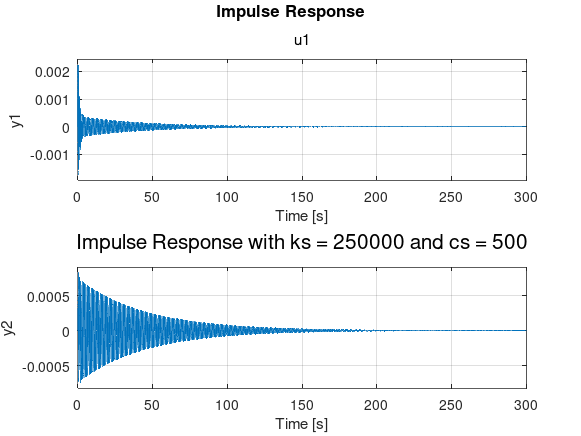
\includegraphics[width=.9\linewidth]{ENG204-Assignment-2-Impulse-Response-111.png}
\end{center}
22nd system:
\begin{center}
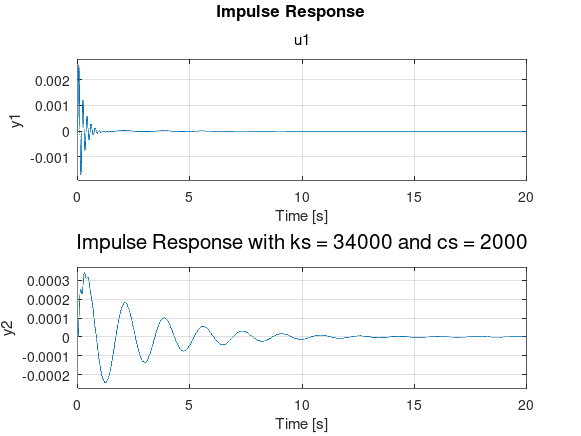
\includegraphics[width=.9\linewidth]{ENG204-Assignment-2-Impulse-Response-22.png}
\end{center}
11th system:
\begin{center}
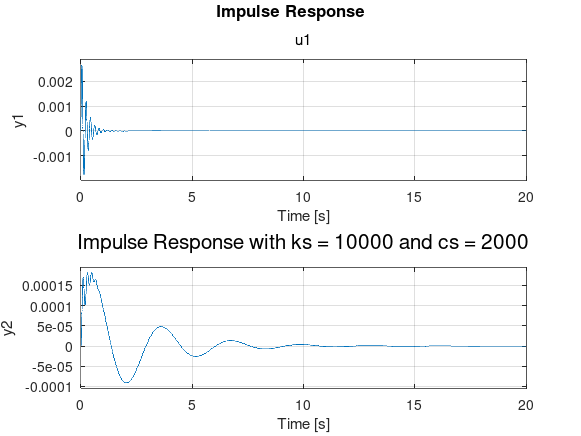
\includegraphics[width=.9\linewidth]{ENG204-Assignment-2-Impulse-Response-11.png}
\end{center}
From these graphs we can see that having a high \(k_s\) and a low \(c_s\) resuts in a slow convergence and very high frequencies. Where as having a low \(k_s\) and high \(c_s\) results in a faster convergence at low frequency. However there is a sweet spot between both where the best response is gathered, which can be seen in the 11th response.
\subsubsection{Stability}
\label{sec:org6a1b386}
Check if the system is stable using the eigenvalues of \(A\).
\begin{minted}[]{octave}
for i = 1:length(sysArray)
    eigen=abs(eig(sysArray(i).A));
    if all(eigen < 1)
        fprintf("The %i th system is stable\n", i)
        maxEig = max(eigen);
        fprintf("The max eigen value is %f\n", maxEig)
    else
        fprintf("The %i th system is unstable\n", i)
    end
end
\end{minted}


This output shows that the system is stable for all \(10,000\leq k_s\leq 250,000 N/m\) and \(500 \leq c_s \leq 2000 Ns/m\). We would also expect to the the most stable system to occur when the largest of the eigenvalues is the smallest, which we can see occurs on the 11th system. The full output can be seen in \hyperref[sec:org5ab6351]{Appendix A}
\subsubsection{Damping}
\label{sec:org77cbc0f}
\begin{minted}[]{octave}
ms=2296;
ksMin = 10000;
csMin = 500;
ksMax = 250000;
csMax = 2000;
idx = 0;
numOfSys = 10;
for i =0:numOfSys;
    for j =0:numOfSys;
        idx = idx +1;
        ks = ksMin + (i/numOfSys)*(ksMax-ksMin);
        cs = csMin + (j/numOfSys)*(csMax-csMin);
        damp = cs / (2 * sqrt(ms * ks));
        fprintf('For the %i th system the damping factor is %f\n', idx, damp)
    end
end
\end{minted}

We want a damping factor of 1, this is when the system will be critically damped. The output shows that the closest to 1 is 0.208696 which occurs on the 11 th system, this aligns with the graphs and eigenvalues. The full output can be seen in \hyperref[sec:org2a10006]{Appendix B}.
\subsection{Part e}
\label{sec:orgdd4ad96}
\subsubsection{Varing Frequency}
\label{sec:orgfb1537d}
The following code is going to use the 11th system, as it has been shown to be the best.
\begin{minted}[]{octave}
fMin=1000;
fStep=fMin;
fMax=10*fMin;
for i = fMin:fStep:fMax
    um = 1;
    f = i; % Frequency
    w0 = 2 * pi * f;
    t = 0:Ts:10;
    u = um * sin(w0 * t);
    figure;
    hold on;
    y = lsim(sys{11}, u, t);
    plot(t, y(:, 2));
    titleStr = sprintf('Response of Quarter-Car Suspension System to Sinusoidal Input at %i Hz', f);
    title(titleStr, 'FontSize', 10);
    xlabel('Time (s)');
    ylabel('Displacement');
    legendEntry = sprintf('System %d: ks = %.2f, cs = %.2f', 11, sysArray(11).ks, sysArray(11).cs);
    legend(legendEntry);
    hold off;
    filename = sprintf('ENG204-Assignment-2-Sinusoidal-f-%i.png', f);
    print(filename,'-dpng','-r100');
end
\end{minted}


Frequencies from 0.1 Hz to 10k Hz were analised. Some samples can be seen here:
\begin{center}
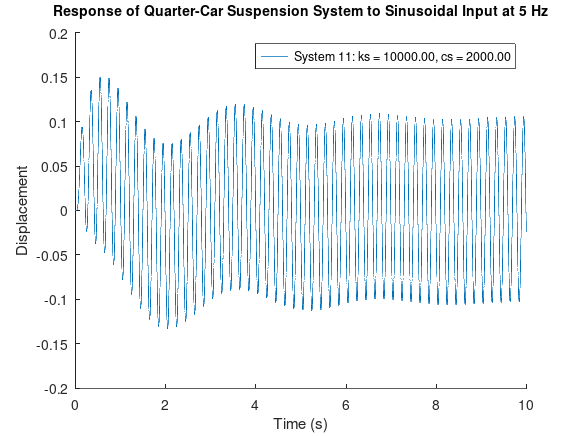
\includegraphics[width=.9\linewidth]{ENG204-Assignment-2-Sinusoidal-f-5.png}
\end{center}
\begin{center}
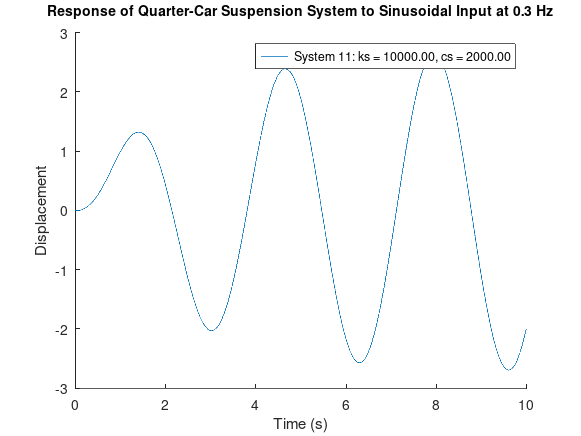
\includegraphics[width=.9\linewidth]{ENG204-Assignment-2-Sinusoidal-f-0.3.png}
\end{center}
\begin{center}
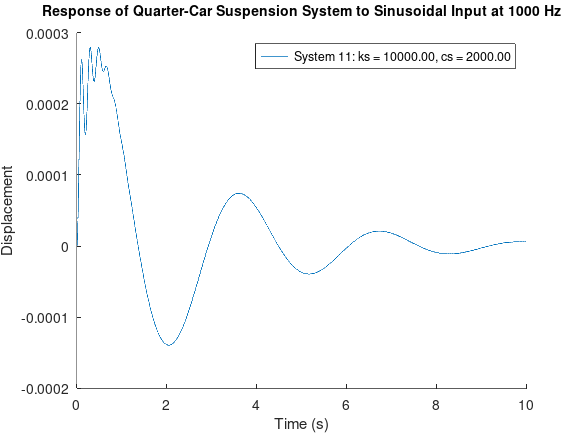
\includegraphics[width=.9\linewidth]{ENG204-Assignment-2-Sinusoidal-f-1000.png}
\end{center}
For low frequencies the vehicle experiences the worst movement, at high frequencies the vehicle experiences very low amount of movement. The worst amplitude occurs at 0.3 Hz, it has a maximum magnitude \(\approx 3\).
\subsubsection{Varing Suspension}
\label{sec:org70c3b0a}
The following code is going to use many systems at 0.3Hz, as it was shown to be the worst for the best case.
\begin{minted}[]{octave}
um = 1;
f = 0.3; % Frequency
w0 = 2 * pi * f;
t = 0:Ts:10;
u = um * sin(w0 * t);

for i = 1:length(sys)
    figure;
    hold on;
    y = lsim(sys{i}, u, t);
    plot(t, y(:, 2));

    titleStr = sprintf('%i th System to Sinusoidal Input at %i Hz', i , f);
    title(titleStr, 'FontSize', 10);
    xlabel('Time (s)');
    ylabel('Displacement');
    legendEntry = sprintf('System %d: ks = %.2f, cs = %.2f', i, sysArray(i).ks, sysArray(i).cs);
    legend(legendEntry);
    hold off;
    filename = sprintf('ENG204-Assignment-2-Sinusoidal-f-0.3-%i.png', i);
    print(filename,'-dpng','-r100');
end
\end{minted}

The best preforming system was the last system, this system has the highest \%k\textsubscript{s}\$ and \(c_s\), the magnitude of the output is \(\approx 1.5\). Decreasing the value of \(k_s\) and \(c_s\) tends to increase the magnitdue of the output. Where the worst peforming system was the first one with the lowest \%k\textsubscript{s}\$ and \(c_s\), it has a magnitude of \(\approx 6\).

\begin{center}
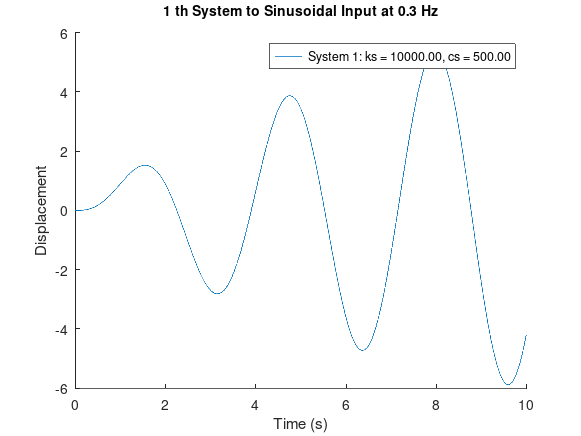
\includegraphics[width=.9\linewidth]{ENG204-Assignment-2-Sinusoidal-f-0.3-1.png}
\end{center}
\begin{center}
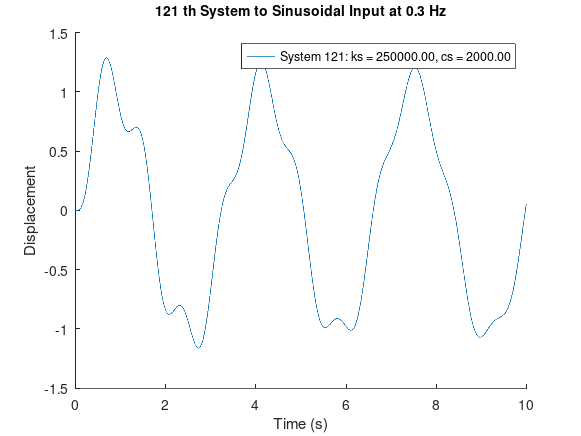
\includegraphics[width=.9\linewidth]{ENG204-Assignment-2-Sinusoidal-f-0.3-121.png}
\end{center}
\subsection{Part f}
\label{sec:org5621049}
The metrics involved in these calculations depend heavily on the use-case of the suspension system being designed. We will assume that the system is designed for general consumer usage, with typical speeds varying from 50km/h to 110km/h(13.8889 to 30.5556 m/s). These speeds impact the frequency of the oscillations as well as the peak suspension displacements. This will lead to varying vehicle smoothness depending on the speed as well as the suspension configuration( ks and cs values). The graphical demonstration developed through MATLAB shows clearly that as the speed increases the amplitude decreases and the frequency increases. This is due to the relationship between frequency and velocity, \(\omega =2\pi v/\lambda\). Where \(\lambda\) is the wavelength of the road bumps. Many documentations have been made on this topic, with varying approaches based on the specific vehicle and usage scenarios.

(??, ????)
\newpage
\begin{LATEX}
\printbibliography
\end{LATEX}
\newpage
\subsection{Appendix A}
\label{sec:org5ab6351}
The 1 th system is stable \\
The max eigen value is 0.999990 \\
The 2 th system is stable \\
The max eigen value is 0.999987 \\
The 3 th system is stable \\
The max eigen value is 0.999984 \\
The 4 th system is stable \\
The max eigen value is 0.999981 \\
The 5 th system is stable \\
The max eigen value is 0.999978 \\
The 6 th system is stable \\
The max eigen value is 0.999975 \\
The 7 th system is stable \\
The max eigen value is 0.999972 \\
The 8 th system is stable \\
The max eigen value is 0.999969 \\
The 9 th system is stable \\
The max eigen value is 0.999966 \\
The 10 th system is stable \\
The max eigen value is 0.999963 \\
The 11 th system is stable \\
The max eigen value is 0.999960 \\
The 12 th system is stable \\
The max eigen value is 0.999992 \\
The 13 th system is stable \\
The max eigen value is 0.999989 \\
The 14 th system is stable \\
The max eigen value is 0.999987 \\
The 15 th system is stable \\
The max eigen value is 0.999984 \\
The 16 th system is stable \\
The max eigen value is 0.999982 \\
The 17 th system is stable \\
The max eigen value is 0.999979 \\
The 18 th system is stable \\
The max eigen value is 0.999976 \\
The 19 th system is stable \\
The max eigen value is 0.999974 \\
The 20 th system is stable \\
The max eigen value is 0.999971 \\
The 21 th system is stable \\
The max eigen value is 0.999969 \\
The 22 th system is stable \\
The max eigen value is 0.999966 \\
The 23 th system is stable \\
The max eigen value is 0.999993 \\
The 24 th system is stable \\
The max eigen value is 0.999991 \\
The 25 th system is stable \\
The max eigen value is 0.999989 \\
The 26 th system is stable \\
The max eigen value is 0.999987 \\
The 27 th system is stable \\
The max eigen value is 0.999984 \\
The 28 th system is stable \\
The max eigen value is 0.999982 \\
The 29 th system is stable \\
The max eigen value is 0.999980 \\
The 30 th system is stable \\
The max eigen value is 0.999978 \\
The 31 th system is stable \\
The max eigen value is 0.999976 \\
The 32 th system is stable \\
The max eigen value is 0.999974 \\
The 33 th system is stable \\
The max eigen value is 0.999972 \\
The 34 th system is stable \\
The max eigen value is 0.999994 \\
The 35 th system is stable \\
The max eigen value is 0.999992 \\
The 36 th system is stable \\
The max eigen value is 0.999990 \\
The 37 th system is stable \\
The max eigen value is 0.999989 \\
The 38 th system is stable \\
The max eigen value is 0.999987 \\
The 39 th system is stable \\
The max eigen value is 0.999985 \\
The 40 th system is stable \\
The max eigen value is 0.999983 \\
The 41 th system is stable \\
The max eigen value is 0.999981 \\
The 42 th system is stable \\
The max eigen value is 0.999980 \\
The 43 th system is stable \\
The max eigen value is 0.999978 \\
The 44 th system is stable \\
The max eigen value is 0.999976 \\
The 45 th system is stable \\
The max eigen value is 0.999995 \\
The 46 th system is stable \\
The max eigen value is 0.999993 \\
The 47 th system is stable \\
The max eigen value is 0.999992 \\
The 48 th system is stable \\
The max eigen value is 0.999990 \\
The 49 th system is stable \\
The max eigen value is 0.999989 \\
The 50 th system is stable \\
The max eigen value is 0.999987 \\
The 51 th system is stable \\
The max eigen value is 0.999986 \\
The 52 th system is stable \\
The max eigen value is 0.999984 \\
The 53 th system is stable \\
The max eigen value is 0.999982 \\
The 54 th system is stable \\
The max eigen value is 0.999981 \\
The 55 th system is stable \\
The max eigen value is 0.999979 \\
The 56 th system is stable \\
The max eigen value is 0.999996 \\
The 57 th system is stable \\
The max eigen value is 0.999994 \\
The 58 th system is stable \\
The max eigen value is 0.999993 \\
The 59 th system is stable \\
The max eigen value is 0.999992 \\
The 60 th system is stable \\
The max eigen value is 0.999990 \\
The 61 th system is stable \\
The max eigen value is 0.999989 \\
The 62 th system is stable \\
The max eigen value is 0.999987 \\
The 63 th system is stable \\
The max eigen value is 0.999986 \\
The 64 th system is stable \\
The max eigen value is 0.999985 \\
The 65 th system is stable \\
The max eigen value is 0.999983 \\
The 66 th system is stable \\
The max eigen value is 0.999982 \\
The 67 th system is stable \\
The max eigen value is 0.999996 \\
The 68 th system is stable \\
The max eigen value is 0.999995 \\
The 69 th system is stable \\
The max eigen value is 0.999994 \\
The 70 th system is stable \\
The max eigen value is 0.999993 \\
The 71 th system is stable \\
The max eigen value is 0.999991 \\
The 72 th system is stable \\
The max eigen value is 0.999990 \\
The 73 th system is stable \\
The max eigen value is 0.999989 \\
The 74 th system is stable \\
The max eigen value is 0.999988 \\
The 75 th system is stable \\
The max eigen value is 0.999987 \\
The 76 th system is stable \\
The max eigen value is 0.999985 \\
The 77 th system is stable \\
The max eigen value is 0.999984 \\
The 78 th system is stable \\
The max eigen value is 0.999997 \\
The 79 th system is stable \\
The max eigen value is 0.999996 \\
The 80 th system is stable \\
The max eigen value is 0.999995 \\
The 81 th system is stable \\
The max eigen value is 0.999994 \\
The 82 th system is stable \\
The max eigen value is 0.999992 \\
The 83 th system is stable \\
The max eigen value is 0.999991 \\
The 84 th system is stable \\
The max eigen value is 0.999990 \\
The 85 th system is stable \\
The max eigen value is 0.999989 \\
The 86 th system is stable \\
The max eigen value is 0.999988 \\
The 87 th system is stable \\
The max eigen value is 0.999987 \\
The 88 th system is stable \\
The max eigen value is 0.999986 \\
The 89 th system is stable \\
The max eigen value is 0.999997 \\
The 90 th system is stable \\
The max eigen value is 0.999996 \\
The 91 th system is stable \\
The max eigen value is 0.999995 \\
The 92 th system is stable \\
The max eigen value is 0.999994 \\
The 93 th system is stable \\
The max eigen value is 0.999993 \\
The 94 th system is stable \\
The max eigen value is 0.999992 \\
The 95 th system is stable \\
The max eigen value is 0.999991 \\
The 96 th system is stable \\
The max eigen value is 0.999991 \\
The 97 th system is stable \\
The max eigen value is 0.999990 \\
The 98 th system is stable \\
The max eigen value is 0.999989 \\
The 99 th system is stable \\
The max eigen value is 0.999988 \\
The 100 th system is stable \\
The max eigen value is 0.999997 \\
The 101 th system is stable \\
The max eigen value is 0.999997 \\
The 102 th system is stable \\
The max eigen value is 0.999996 \\
The 103 th system is stable \\
The max eigen value is 0.999995 \\
The 104 th system is stable \\
The max eigen value is 0.999994 \\
The 105 th system is stable \\
The max eigen value is 0.999993 \\
The 106 th system is stable \\
The max eigen value is 0.999992 \\
The 107 th system is stable \\
The max eigen value is 0.999992 \\
The 108 th system is stable \\
The max eigen value is 0.999991 \\
The 109 th system is stable \\
The max eigen value is 0.999990 \\
The 110 th system is stable \\
The max eigen value is 0.999989 \\
The 111 th system is stable \\
The max eigen value is 0.999998 \\
The 112 th system is stable \\
The max eigen value is 0.999997 \\
The 113 th system is stable \\
The max eigen value is 0.999996 \\
The 114 th system is stable \\
The max eigen value is 0.999995 \\
The 115 th system is stable \\
The max eigen value is 0.999995 \\
The 116 th system is stable \\
The max eigen value is 0.999994 \\
The 117 th system is stable \\
The max eigen value is 0.999993 \\
The 118 th system is stable \\
The max eigen value is 0.999992 \\
The 119 th system is stable \\
The max eigen value is 0.999992 \\
The 120 th system is stable \\
The max eigen value is 0.999991 \\
The 121 th system is stable \\
The max eigen value is 0.999990 \\

\newpage
\subsection{Appendix B}
\label{sec:org2a10006}
For the 1 th system the damping factor is 0.052174 \\
For the 2 th system the damping factor is 0.067826 \\
For the 3 th system the damping factor is 0.083478 \\
For the 4 th system the damping factor is 0.099131 \\
For the 5 th system the damping factor is 0.114783 \\
For the 6 th system the damping factor is 0.130435 \\
For the 7 th system the damping factor is 0.146087 \\
For the 8 th system the damping factor is 0.161739 \\
For the 9 th system the damping factor is 0.177392 \\
For the 10 th system the damping factor is 0.193044 \\
For the 11 th system the damping factor is 0.208696 \\
For the 12 th system the damping factor is 0.028295 \\
For the 13 th system the damping factor is 0.036784 \\
For the 14 th system the damping factor is 0.045273 \\
For the 15 th system the damping factor is 0.053761 \\
For the 16 th system the damping factor is 0.062250 \\
For the 17 th system the damping factor is 0.070738 \\
For the 18 th system the damping factor is 0.079227 \\
For the 19 th system the damping factor is 0.087715 \\
For the 20 th system the damping factor is 0.096204 \\
For the 21 th system the damping factor is 0.104693 \\
For the 22 th system the damping factor is 0.113181 \\
For the 23 th system the damping factor is 0.021664 \\
For the 24 th system the damping factor is 0.028163 \\
For the 25 th system the damping factor is 0.034663 \\
For the 26 th system the damping factor is 0.041162 \\
For the 27 th system the damping factor is 0.047661 \\
For the 28 th system the damping factor is 0.054160 \\
For the 29 th system the damping factor is 0.060659 \\
For the 30 th system the damping factor is 0.067159 \\
For the 31 th system the damping factor is 0.073658 \\
For the 32 th system the damping factor is 0.080157 \\
For the 33 th system the damping factor is 0.086656 \\
For the 34 th system the damping factor is 0.018220 \\
For the 35 th system the damping factor is 0.023686 \\
For the 36 th system the damping factor is 0.029152 \\
For the 37 th system the damping factor is 0.034618 \\
For the 38 th system the damping factor is 0.040084 \\
For the 39 th system the damping factor is 0.045550 \\
For the 40 th system the damping factor is 0.051016 \\
For the 41 th system the damping factor is 0.056482 \\
For the 42 th system the damping factor is 0.061948 \\
For the 43 th system the damping factor is 0.067414 \\
For the 44 th system the damping factor is 0.072880 \\
For the 45 th system the damping factor is 0.016025 \\
For the 46 th system the damping factor is 0.020833 \\
For the 47 th system the damping factor is 0.025640 \\
For the 48 th system the damping factor is 0.030448 \\
For the 49 th system the damping factor is 0.035255 \\
For the 50 th system the damping factor is 0.040063 \\
For the 51 th system the damping factor is 0.044870 \\
For the 52 th system the damping factor is 0.049678 \\
For the 53 th system the damping factor is 0.054485 \\
For the 54 th system the damping factor is 0.059293 \\
For the 55 th system the damping factor is 0.064100 \\
For the 56 th system the damping factor is 0.014470 \\
For the 57 th system the damping factor is 0.018812 \\
For the 58 th system the damping factor is 0.023153 \\
For the 59 th system the damping factor is 0.027494 \\
For the 60 th system the damping factor is 0.031835 \\
For the 61 th system the damping factor is 0.036176 \\
For the 62 th system the damping factor is 0.040517 \\
For the 63 th system the damping factor is 0.044858 \\
For the 64 th system the damping factor is 0.049200 \\
For the 65 th system the damping factor is 0.053541 \\
For the 66 th system the damping factor is 0.057882 \\
For the 67 th system the damping factor is 0.013295 \\
For the 68 th system the damping factor is 0.017284 \\
For the 69 th system the damping factor is 0.021272 \\
For the 70 th system the damping factor is 0.025261 \\
For the 71 th system the damping factor is 0.029249 \\
For the 72 th system the damping factor is 0.033238 \\
For the 73 th system the damping factor is 0.037226 \\
For the 74 th system the damping factor is 0.041215 \\
For the 75 th system the damping factor is 0.045204 \\
For the 76 th system the damping factor is 0.049192 \\
For the 77 th system the damping factor is 0.053181 \\
For the 78 th system the damping factor is 0.012366 \\
For the 79 th system the damping factor is 0.016076 \\
For the 80 th system the damping factor is 0.019786 \\
For the 81 th system the damping factor is 0.023496 \\
For the 82 th system the damping factor is 0.027206 \\
For the 83 th system the damping factor is 0.030916 \\
For the 84 th system the damping factor is 0.034626 \\
For the 85 th system the damping factor is 0.038336 \\
For the 86 th system the damping factor is 0.042046 \\
For the 87 th system the damping factor is 0.045756 \\
For the 88 th system the damping factor is 0.049466 \\
For the 89 th system the damping factor is 0.011609 \\
For the 90 th system the damping factor is 0.015091 \\
For the 91 th system the damping factor is 0.018574 \\
For the 92 th system the damping factor is 0.022056 \\
For the 93 th system the damping factor is 0.025539 \\
For the 94 th system the damping factor is 0.029021 \\
For the 95 th system the damping factor is 0.032504 \\
For the 96 th system the damping factor is 0.035987 \\
For the 97 th system the damping factor is 0.039469 \\
For the 98 th system the damping factor is 0.042952 \\
For the 99 th system the damping factor is 0.046434 \\
For the 100 th system the damping factor is 0.010975 \\
For the 101 th system the damping factor is 0.014267 \\
For the 102 th system the damping factor is 0.017560 \\
For the 103 th system the damping factor is 0.020852 \\
For the 104 th system the damping factor is 0.024145 \\
For the 105 th system the damping factor is 0.027437 \\
For the 106 th system the damping factor is 0.030730 \\
For the 107 th system the damping factor is 0.034022 \\
For the 108 th system the damping factor is 0.037315 \\
For the 109 th system the damping factor is 0.040607 \\
For the 110 th system the damping factor is 0.043900 \\
For the 111 th system the damping factor is 0.010435 \\
For the 112 th system the damping factor is 0.013565 \\
For the 113 th system the damping factor is 0.016696 \\
For the 114 th system the damping factor is 0.019826 \\
For the 115 th system the damping factor is 0.022957 \\
For the 116 th system the damping factor is 0.026087 \\
For the 117 th system the damping factor is 0.029217 \\
For the 118 th system the damping factor is 0.032348 \\
For the 119 th system the damping factor is 0.035478 \\
For the 120 th system the damping factor is 0.038609 \\
For the 121 th system the damping factor is 0.041739 \\
\end{document}
